\documentclass{article}
\pagestyle{empty}
\usepackage[utf8]{inputenc}
\usepackage{tikz}
\usetikzlibrary{shapes.geometric, arrows}

\tikzstyle{box} = [rectangle, rounded corners, minimum width=3cm, minimum height=1cm,text centered, draw=black, thick, fill=green!30]
\tikzstyle{redBox} = [rectangle, rounded corners, minimum width=3cm, minimum height=1cm,text centered, draw=black, thick, fill=red!30]
\tikzstyle{yellowBox} = [rectangle, rounded corners, minimum width=3cm, minimum height=1cm, text centered, draw=black, thick, fill=yellow!30]
\tikzstyle{yellowBoxRedBorder} = [rectangle, rounded corners, minimum width=3cm, minimum height=1cm, text centered, draw=red, thick, fill=yellow!30]
\tikzstyle{plainBox} = [rectangle, rounded corners, minimum width=3cm, minimum height=1cm, text centered, draw=black, thick]
\tikzstyle{plainBoxRedBorder} = [rectangle, rounded corners, minimum width=3cm, minimum height=1cm, text centered, draw=red,thick]
\tikzstyle{dataBox} = [rectangle, rounded corners, minimum width=8.0cm, minimum height=4.1cm,text centered, draw=black,thick, fill=gray!10]
\tikzstyle{invariantBox} = [rectangle, rounded corners, minimum width=4.7cm, minimum height=8.1cm,text centered, draw=black,thick, fill=blue!10]
\tikzstyle{arrow} = [thick,->,>=stealth]

\begin{document}

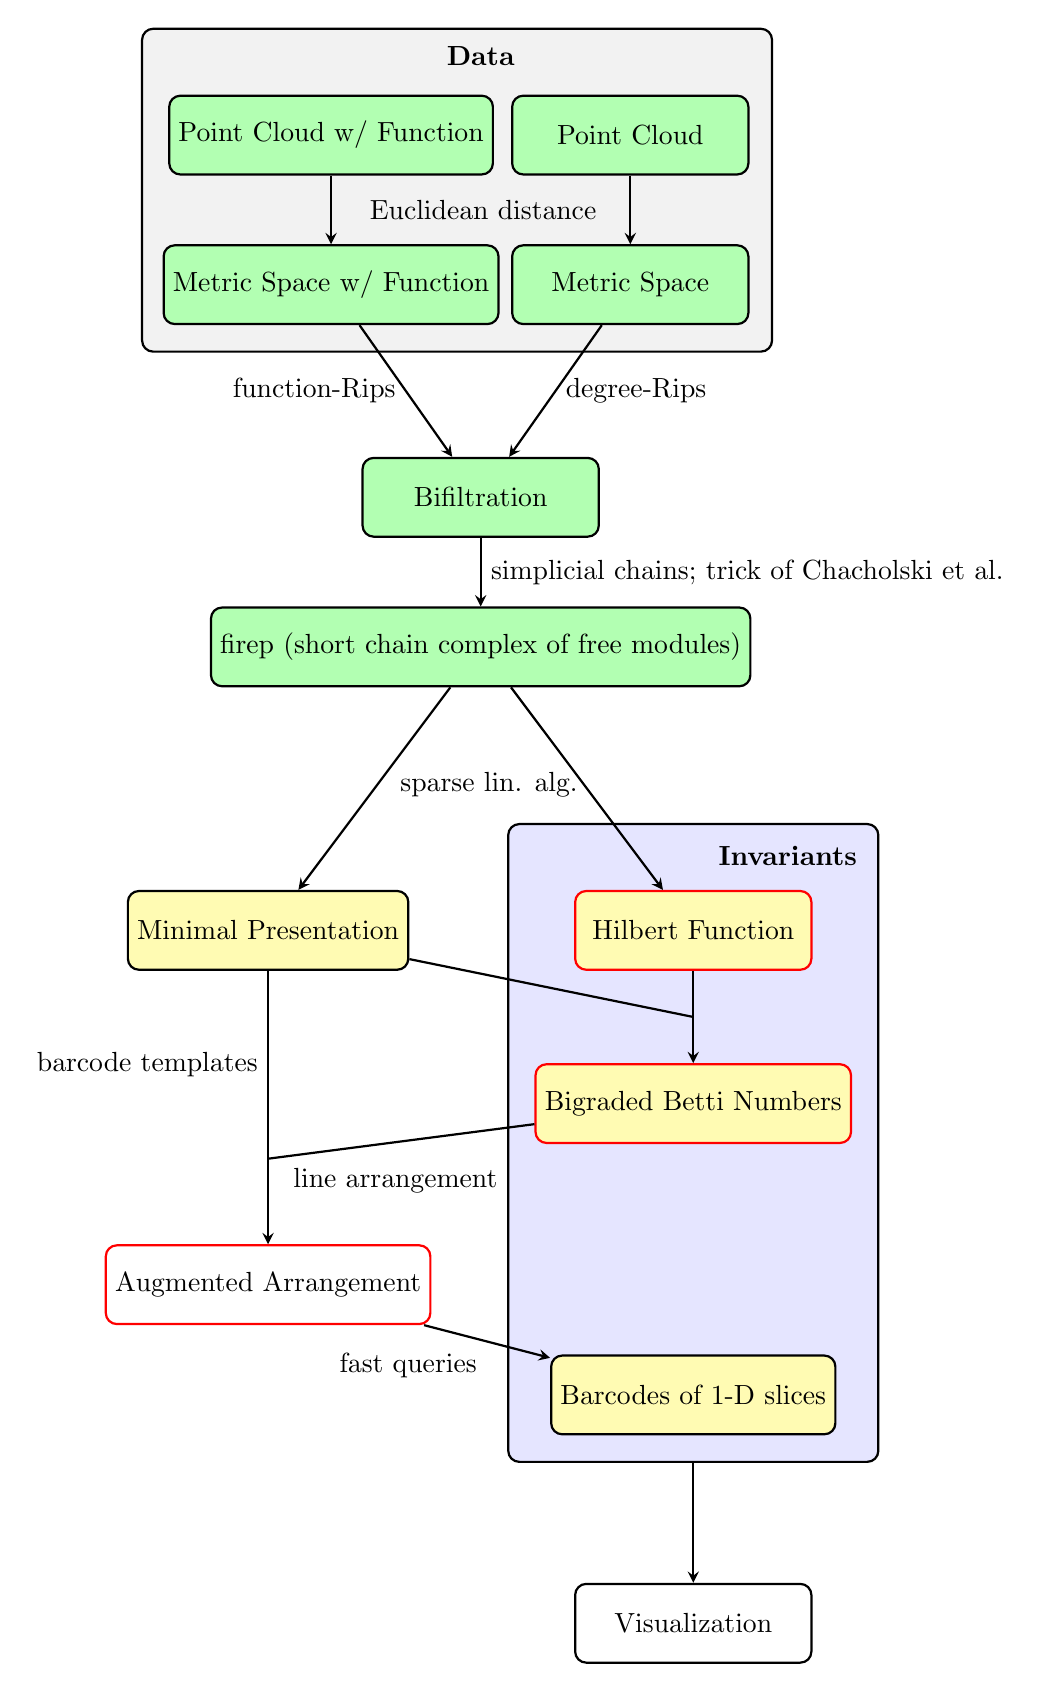
\begin{tikzpicture}[node distance=1.9cm]

\node (pointsAnchor) [yshift = -1cm] {};
\node (data) [dataBox,yshift=-1.7cm,xshift=-.3cm] {};
\node (dataLabel) {\textbf{Data}};
\node (metricAnchor) [below of= pointsAnchor] {};
\node (pointsFun) [box,left of=pointsAnchor] {Point Cloud w/ Function};
\node (points) [box,right of=pointsAnchor] {Point Cloud};
\node (metricFun) [box,left of=metricAnchor] {Metric Space w/ Function};
\node (metric) [box,right of=metricAnchor] {Metric Space};
\node (bifiltration) [box, below of=metricAnchor,yshift=-.8cm] {Bifiltration};
%\node (input) [yellowBox,left of= bifiltration, xshift=-5cm] {Text File Input};
\node (firep) [box, below of=bifiltration] {firep (short chain complex of free modules)};
\node (magicAnchor) [below of= firep,yshift=-1.7cm] {};
\node (minpres) [yellowBox, left of=magicAnchor,xshift=-.8cm] {Minimal Presentation};
\node (invariant) [invariantBox,right of= magicAnchor,xshift=.8cm,yshift=-2.7cm] {};
\node (invariantLabel) [right of= magicAnchor,xshift=2.0cm,yshift=.95cm] {\textbf{Invariants}};
\node (hilbert)[yellowBoxRedBorder, right of= magicAnchor,xshift=.8cm]{Hilbert Function};
\node (bettiCombine) [coordinate,below of= hilbert,yshift=.8cm] {};
\node (betti) [yellowBoxRedBorder, below of= bettiCombine,yshift=.8cm]{Bigraded Betti Numbers};
\node (arrangementCombine)[coordinate, below of= minpres,yshift=-1cm] {};
\node (arrangement)[plainBoxRedBorder, below of= arrangementCombine,yshift=.3cm] {Augmented Arrangement};
\node (barcodes)[yellowBox, below of= hilbert, yshift=-4cm]  {Barcodes of 1-D slices};
\node (visualization)[plainBox, below of= barcodes,yshift=-1cm]  {Visualization};
%\node (minpres) [box, below of=firep, yshift=-0.5cm] {Minimal Presentation};
%\node (pro2a) [process, below of=minpres, yshift=-0.5cm] {};
%\node (pro2b) [process, right of=minpres, xshift=2cm] {Process 2b};
%\node (out1) [io, below of=pro2a] {Output};
%\node (stop) [box, below of=out1] {Stop};
%\draw [arrow] (input) -- (data);
%\draw [arrow] (input) -- (bifiltration);
%\draw [arrow] (input) -- (firep);
\draw [arrow] (points) --  node[anchor=east,xshift=-0.3cm]{Euclidean distance} (metric);
\draw [arrow] (pointsFun) --  (metricFun);
\draw [arrow] (metric) -- node[anchor=west]{degree-Rips}(bifiltration);
\draw [arrow] (metricFun) -- node[anchor=east]{function-Rips} (bifiltration);
\draw [arrow] (bifiltration) -- node[anchor=west]{simplicial chains; trick of Chacholski et al.} (firep);
\draw [arrow] (firep) -- node[anchor=west,xshift=.2cm,yshift=.05cm]{sparse lin. alg.} (minpres);
\draw [arrow] (firep) -- (hilbert);
\draw [thick] (minpres) -- (bettiCombine);
\draw [thick] (hilbert) -- (bettiCombine);
\draw [arrow] (bettiCombine) -- (betti);
\draw [thick] (betti) -- node[anchor=west,xshift=-1.5cm,yshift=-.5cm]{line arrangement}(arrangementCombine);
\draw [thick] (minpres) -- node[anchor=east]{barcode templates}(arrangementCombine);
\draw [arrow] (arrangementCombine) -- (arrangement);
\draw [arrow] (invariant) -- (visualization);
%\draw [arrow] (minpres) -- node[anchor=east] {yes} (pro2a);
%\draw [arrow] (minpres) -- node[anchor=south] {no} (pro2b);
%\draw [arrow] (pro2b) |- (firep);
%\draw [arrow] (pro2a) -- (out1);
%\draw [arrow] (out1) -- (stop);

\draw [arrow] (arrangement) -- node[anchor=east,yshift=-.3cm]{fast queries} (barcodes);
\end{tikzpicture}

\end{document}